\section{Ergebnisse}
    
    \subsection{Bewertung des Systems}
        \label{sec:bewerten_des_systems}
        Um den entstandenen Maprotagenerator bewerten zu können und den Grad der Qualität festellen zu können, 
        werden die Metriken aus Kapitel \ref{} \todo{ref} zur Hilfe genommen. Die Metriken sind für Squadmaprotas
        allgemeingültig und anhand dessen könnten sie miteinader verglichen werden. Es soll nicht unerwähnt bleiben,
        dass durch eine schlechte oder auch falsche Wahl der Einstellparameter das Maprotasystem leicht bis hin zu 
        sehr stark beeinträchtigen werden kann. Genaueres dazu ist unter \ref{s:grenzen_des_systems} nachzulesen.
        Daher ist bei diese Bewertung zu berücksichtigen, dass von uns wohl überlegte Einstellparameter festgelegt wurden
        und als Referenz für Änderungen herangezogen werden sollten.
        Das Wählen passender Einstellparameter kann in User manual nachgelesen werden.
   
        Es folgt die Auswertung der Maprota anhand der vorgegebenen Werten.\\

        \subsubsection{Mapverteilung}
            Die Mapverteilung wird von den Layervotes beeinflusst, dieses ist in Kapitel \ref{} \todo{ref} nachzulesen.
            Diese Verteilung ist die Vorgabe für das System und dieses versucht es optimal anzunähern. Da durch die 
            Zielvorgaben die Verteilungsvorgabe nicht immer erreicht werden kann, tritt ein Abweichung in der Verteilung auf.
            Diese Abweichung wird hier als mittlere quadratische Abweichung (MSD) \todo{ac?} pro Modus angegeben.
            Für diese Auswertung wurden den Verteilungen genommen, die aus den Layervotes vom 19.09.2022 entstanden sind.
            Dabei ist zu beachten, dass der Modus TC zu diesem Zeitpunkt \glqq{}Verbugged\grqq{} ist und daher 
            in der Tabelle \ref{t:Ergebnisse:fehler_Mapverteilung} nicht auftaucht.\\
            \begin{table}[h]
                \centering
                \begin{tabular}{|| c c ||}
                    \hline
                    Modus & MSD \\
                    \hline
                    \hline
                    RAAS & 0.00192 \\
                    \hline
                    AAS & 0.00090 \\
                    \hline
                    Invasion & 0.00336 \\
                    \hline
                    Insurgency & 0.00836 \\
                    \hline
                    Destruction & 0.04831 \\
                    \hline
                \end{tabular}
                \caption{mittlere quadratische Abweichung Mapverteilung}
                \label{t:Ergebnisse:fehler_Mapverteilung}
            \end{table}
            
            Um eine Vorstellung zu Entwickeln wird im Folgenden die angestrebte und generierte Verteilung als 
            Diagramm dargestellt (siehe Abbildung \ref{fig:expected_mapverteilung_raas} 
            und Abbildung \ref{fig:generated_mapverteilung_raas}).

            \begin{figure}[h]
                \centering
                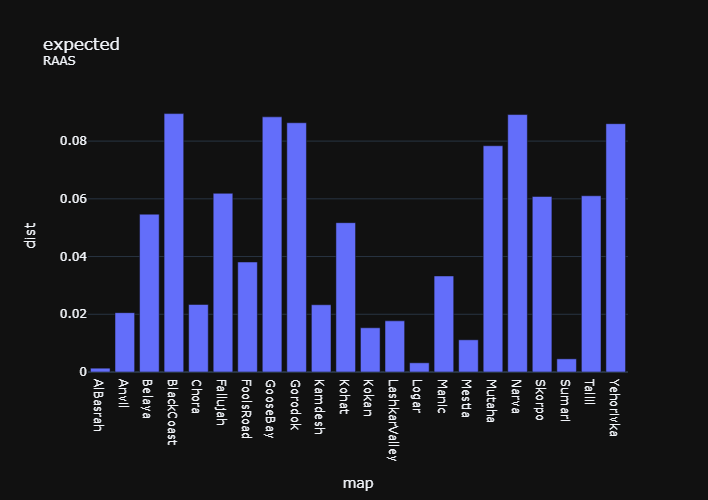
\includegraphics[width=0.7\textwidth]{RAAS_expected.png}
                \caption{erwartete Mapverteilung im Modus RAAS nach den Layervotes vom 19.09.2022}
                \label{fig:expected_mapverteilung_raas}
            \end{figure}

            \begin{figure}[h]
                \centering
                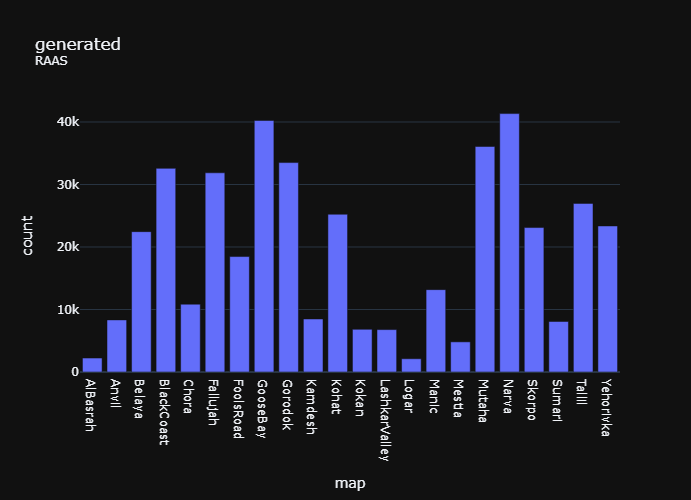
\includegraphics[width=0.7\textwidth]{RAAS_generated.png}
                \caption{generierte Mapverteilung im Modus RAAS nach den Layervotes vom 19.09.2022 (1.Mio. Layer Rota)}
                \label{fig:generated_mapverteilung_raas}
            \end{figure}

            Bei der Betrachtung der Diagramme 
            (Abbildung \ref{fig:expected_mapverteilung_raas} und Abbildung \ref{fig:generated_mapverteilung_raas}) 
            ist zu beachten, dass es sich hier nur um den Modus RAAS handelt.
            Beispielsweise ist die Karte AlBashrah hier deutlich unterrepräsentiert diese ist im Modus Invasion
            nicht der Fall, da die Layervotes dort für AlBashrah deutlich besser ausfallen.
            Zudem lässt sich erkennen, dass die Karte Yehorivka, Blackcoast und Gorodok nicht den angestrebten
            Verteilung erreichen. Dieses Phänomen \ref{s:grenzen_des_systems} näher behandelt.

        \subsubsection{Mode/Modus verteilung}
            Wie bei den Mapverteilungen kann bei den Modusverteilungen die mittlere quadratische Abweichung als
            quantifizierendes Mitteln genommen werden. Bei den Modi ergibt sich eine MSD = $0.04514$.
            Dieser Wert ist für die vorgesehenen Einstellparameter akzeptabel, da Modi die nicht RAAS oder AAS sind
            einen Mindestabstand haben. In diesem Falle ist dieser Abstand 4 Runden.
        \subsubsection{Varriation der Maps}
            Für den die Messbarkeit, der Differenz aufeinander folgende Maps, kann das arithmetische Mittel der Distanzen
            auf der Hyperfläche genutzt werden. Zudem ist es noch sinnvoll sich den gleitenden Mittelwert der Distanzen
            zu betrachten.\\
            Das arithmetische Mittel der Distanzen beträgt $d_m = 1.08946$\\
            \todo{Bewertung das wertes}
            Die Betrachtung des gleitenden Mittelwertes ergibt sich für eine Mittelwertbreite von 5 und einer Rota mit 100000 Layern
            eine Verteilung die auf Abbildung \ref{fig:haufigkeit_gleitender_mittelwert} zu sehen ist.
            
            \begin{figure}[h]
                \centering
                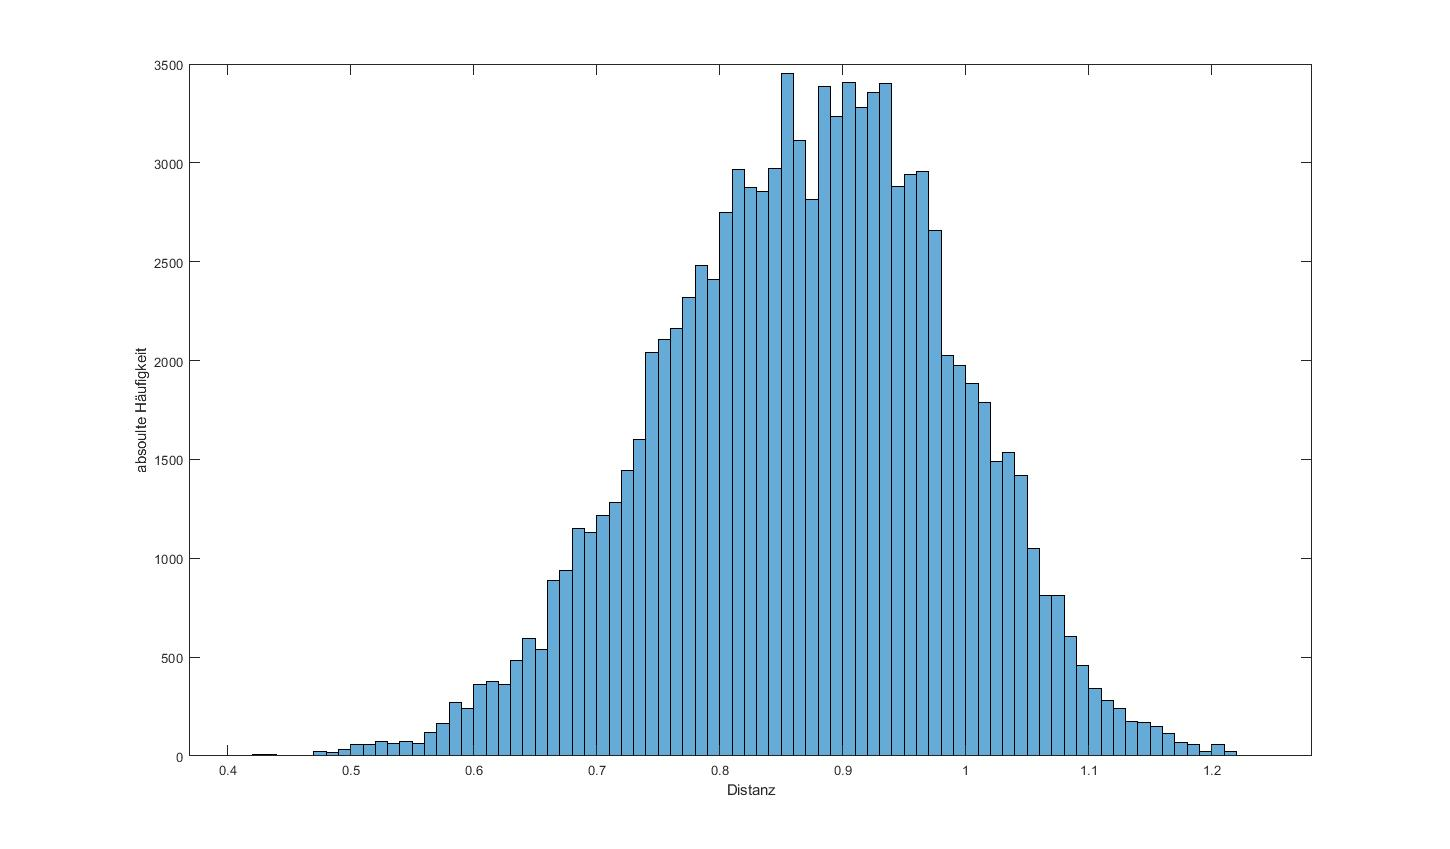
\includegraphics[width=0.9\textwidth]{gleitender_mittelwert_biom_distanz.jpg}
                \caption{Häufigkeiten des gleitenden Mittelwertes der Distanzen}
                \label{fig:haufigkeit_gleitender_mittelwert}
            \end{figure}
            
            \todo{bewertung des histograms}

        \subsubsection{Map Wiederholung}
            Das nächste und hier letzte benutzte Mittel, um eine Maprota zu bewerten ist, nach wie vielen Runden sich eine Map
            wiederholt. Hierfür wurde eine Histogramm aus einer 100000 Layer Rota erstellt.
            Die Abbildung \ref{fig:haufigkeit_der_map_wiederholung} zeigt die Häufigkeit einer Map Wiederholung. Es ergibt sich ein
            Minimum von 3 Runden bevor sich eine Map wiederholen kann. Am Häufigsten ist jedoch eine Map Wiederholung nach 6 bis 9 Runden.
            Dabei muss bedacht werden, das Squad aktuell (09.2022) spielbare Maps beinhaltet. Daher ist dieses ein gutes Wiederholverhalten.

            \begin{figure}[h]
                \centering
                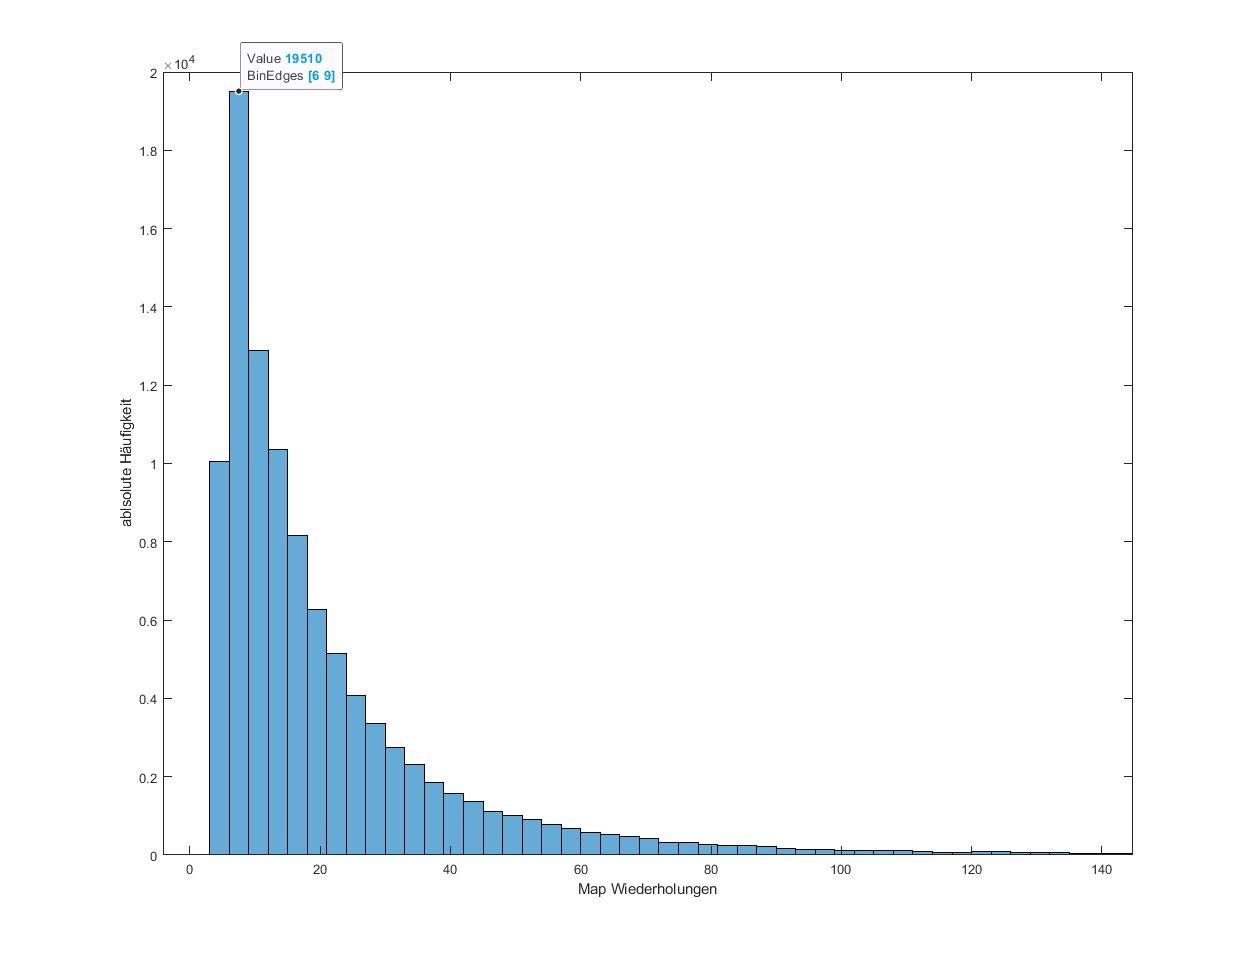
\includegraphics[width=0.9\textwidth]{mapWiederholungsHaufigkeiten.jpg}
                \caption{Häufigkeiten der Map Wiederholung}
                \label{fig:haufigkeit_der_map_wiederholung}
            \end{figure}

        % wie kommt er mit verschiedenen Mapverteilungen klar 
        % Was sind die Einstellungen und warum haben wir so gewählt
    \subsection{Grenzen des Systems}
        \label{s:grenzen_des_systems}
        Um dieses Sektion am besten nachzuvollziehen zu können, sollte nochmal ein Blick auf die Ziele des Systems
        geworfen werden. Es wird eine qualitativ hohe Maprota gefordert, die zum einen der Voteverteilung folgen soll und
        zum anderen in der Map-Reihenfolge einige gewisse Diversität garantieren soll. Bei genauere Überlegung ist
        das schon ein Widerspruch in sich. Angenommen eine einzelne Map hat unendlich viele Stimmen und die Maprota 
        folgt strikt den Votes. Es würde Resultieren, dass nur noch die eine Map drankommen würde. Diese, von 
        der Maprota, angenommene Verteilung bildet aber einen Konflikt mit dem Ziel, dass die Maps eine gewisse Diversität
        bieten sollen. Daher sind an der Stelle die Möglichkeiten das Systems beschränkt und die Voteverteilung kann 
        nicht immer in einer generierten Rota abgebildet werden. Sehr stark hoch gewählte Maps können nur so oft drankommen,
        wie es die Clusterstruktur und die Locktime zulässt. Dieser Aspekt des Systems muss aber nicht als negativer Punkt 
        aufgefasst werden, denn keiner will immer nur eine Map spielen (solange es nicht GooseBay ist). 
        Dieses \glqq{}Feature\glqq{} wirkt damit aktiv gegen die Befürchtung, welche im Feedback-chat angesprochen wurde,
        dass nur noch Yehorivka und Gorodok drankommen.
        Um trotzdem das Optimum zwischen vorgegebener Verteilung und Diversität der Maps zu garantieren wird ein Optimizer
        eingesetzt.\\
        Eine Weitere Grenze des System ist die Falsche Bedienung. Jedes System kann nur so gut sein wie der Anwender*in.
        Damit soll zu Ausdruck gebracht werden, wenn unwissend am System Einstellungen geändert werden, kann die kleinste 
        Änderung alle im Abschnitt \ref{sec:bewerten_des_systems} ungültig machen.\\
        \todo{weitere grenzen ?}
        % warum kann man mit gewissen einstellungen die Rota zu zerstören kann
        % optimizer warum das ? 
